\chapter{Results}\label{ch:results}

This chapter presents the numerical results for the distributions of
topples, area, loss, and length. The selected upper cutoffs for the
power-law analysis are reported in Table~\ref{tab:powerlaw-cutoffs}. For the Manna topples and area distributions, a fixed lower cutoff of $x_{\min}=2$ was used for every system size, excluding the $x=1$ observations associated with the initial plateau. All other power-law fits used $x_{\min}=1$.

\begin{table}[htbp]
    \centering
    \begin{tabular}{lcccccc}\toprule
          Property&Model&  $L=10$&  $L=20$&  $L=30$&  $L=40$& $L=50$\\\midrule
          Topples&BTW&  29&  90&  212&  339& 540\\
          &Manna&  47&  261&  870&  1947& 3288\\ 
 Area& BTW& 27& 78& 177& 269&424\\
 & Manna& 23& 100& 246& 478&721\\ 
 Length& BTW& 8& 15& 24& 32&40\\
 & Manna& 8& 18& 28& 39&50\\ \bottomrule
    \end{tabular}
    \caption{Selected upper cutoffs for the power-law fits. A fixed lower cutoff of $x_{min}=2$ was used for the Manna topples and area distributions; all other fits used  $x_{min}=1$}
    \label{tab:powerlaw-cutoffs}
\end{table}

\section{Topples}\label{sec:topples}

\begin{figure}[htbp]
    \centering
    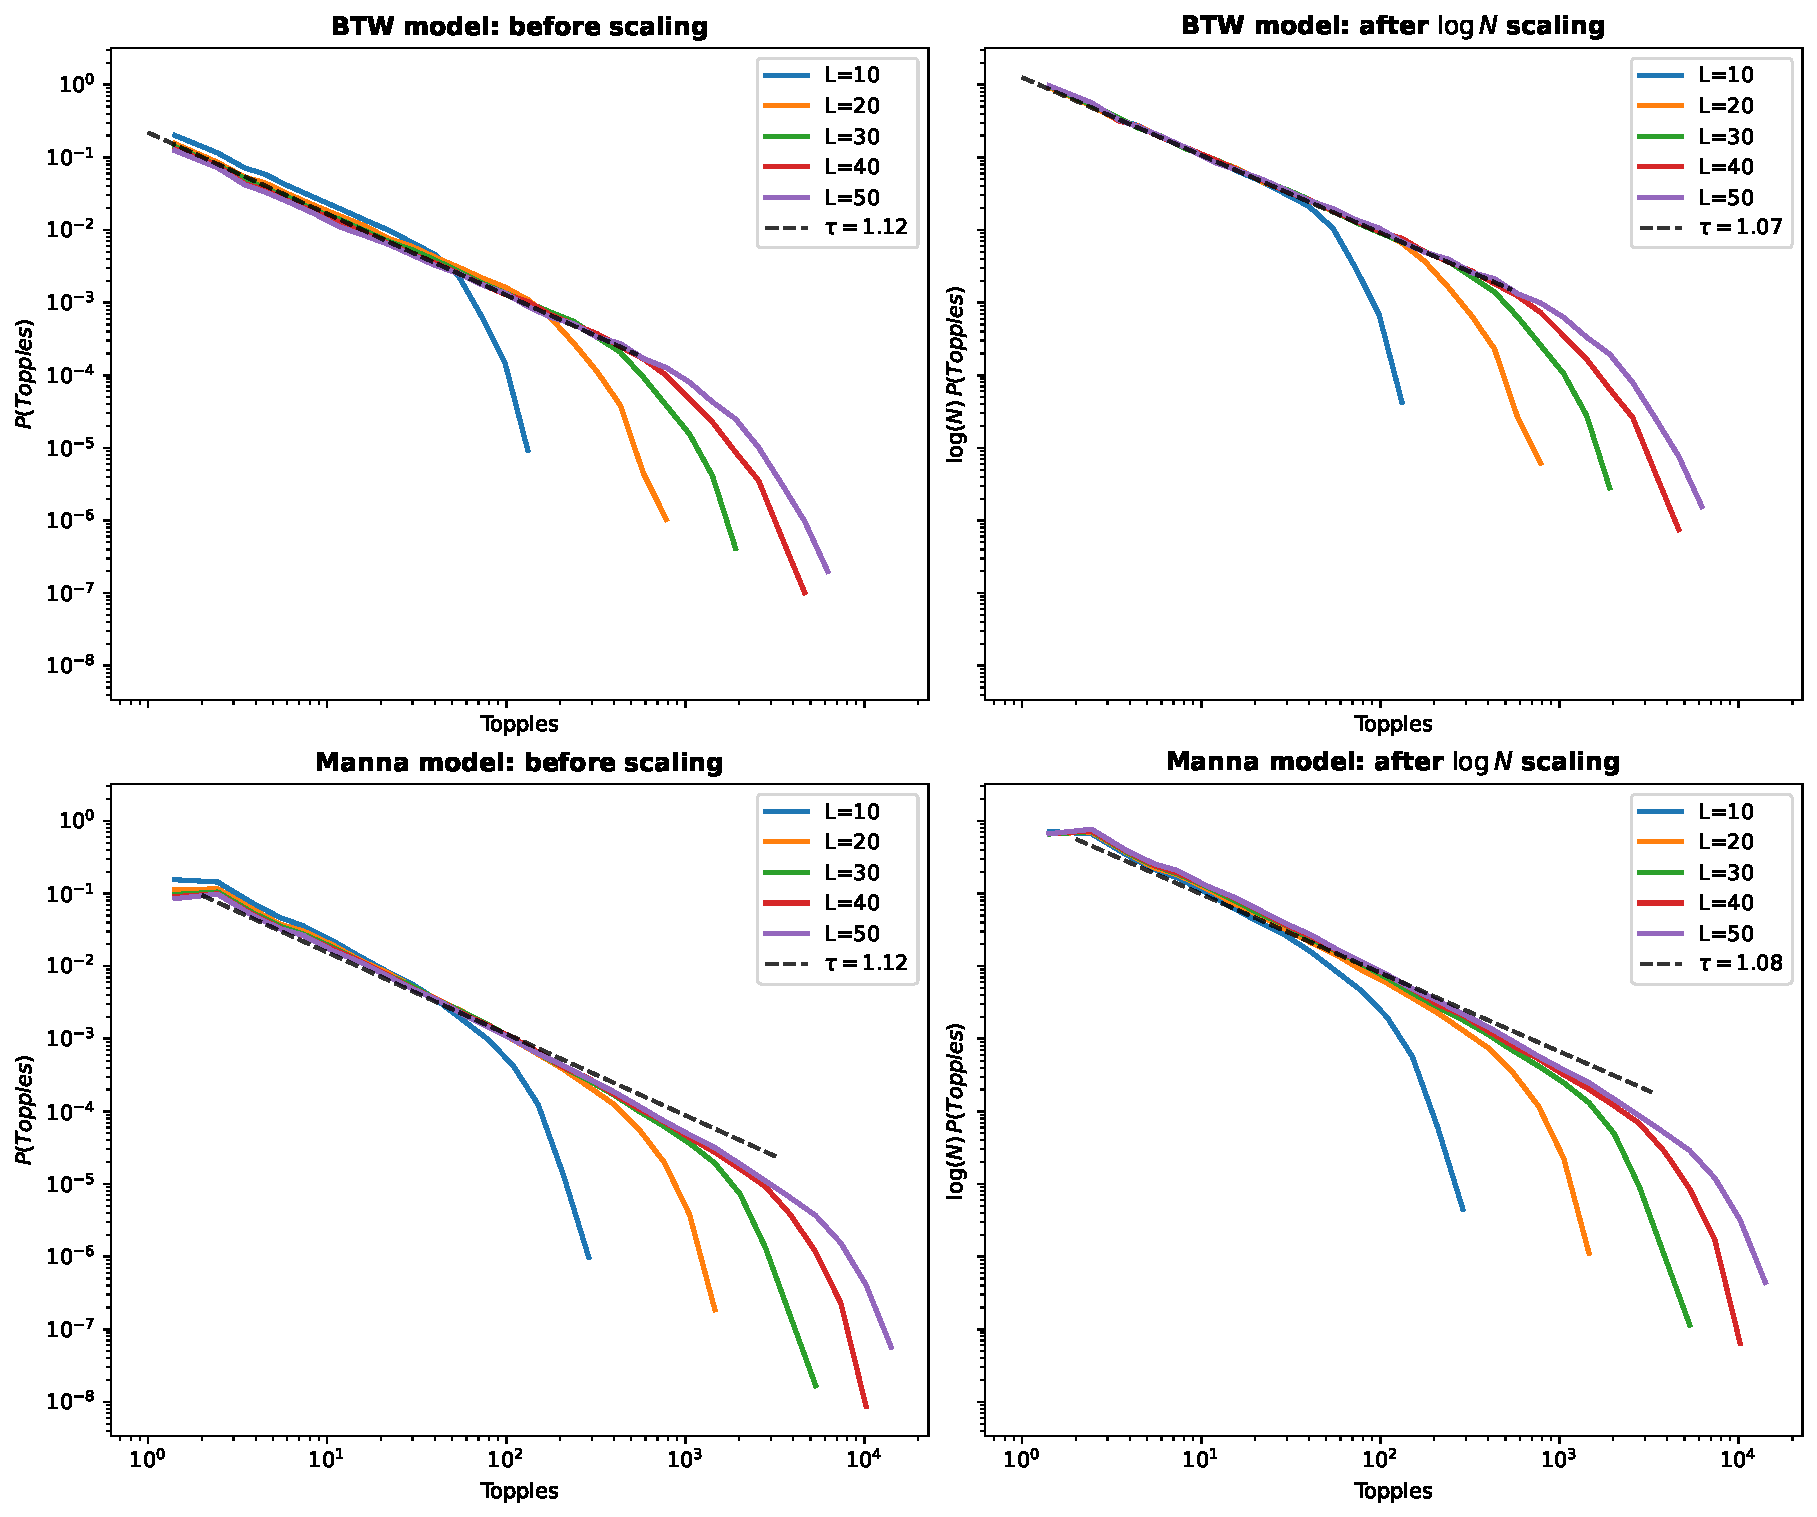
\includegraphics[width=0.80\linewidth]{figures/topples.pdf}
    \caption{Log-binned topples distributions for the BTW model (top row) and Manna model (bottom row), before scaling (left column) and after $\log N$ scaling (right column). Dashed lines show the common power-law fits. }
    \label{fig:topples}
\end{figure}
Figure ~\ref{fig:topples} shows the distributions of the number of topples for the BTW and Manna models, before and after $\log N$ scaling. For both models, the distributions exhibit an approximately straight segment on log-log axes, followed by a system size dependent tail. The tail reaches to larger topples values as $L$ increases, indicating a finite-size cutoff. 

\begin{table}[htbp]
    \centering
    \begin{tabular}{cccc}\toprule
         Model&  $\log N$ scaling&  $\tau$& Overall RMSE\\\midrule
         BTW&  before&  1.120& 0.311\\
         &  after&  1.070& 0.299\\
         Manna&  before&  1.123& 0.478\\
         &  after&  1.084& 0.491\\ \bottomrule
    \end{tabular}
    \caption{Common power-law exponent estimates and overall RMSEs (in log scale) for the topples distributions. }
    \label{tab:topples-summary}
\end{table}

For the BTW model, the common fit before $\log N$ scaling is $\tau_s=1.120$, compared to $\tau_s'=1.070$ after the scaling. The overall RMSE decreases from 0.311 to 0.299, corresponding to a slight reduction. For the Manna model, the corresponding exponents are 1.123 and 1.084 respectively, which lie very close to the BTW estimates. In contrast, the overall RMSE changes from 0.478 to 0.491, a slight increase.\\
\begin{table}[htbp]
    \centering
    \begin{tabular}{cccclll}\toprule
         Model&  $\log N$ scaling&  $L=10$&  $L=20$& $L=30$& $L=40$& $L=50$\\\midrule
         BTW&  before&  0.449&  0.504& 0.609& 1.068& 1.900\\
         &  after&  0.310&  0.327& 0.610& 1.080& 1.879\\
         Manna&  before&  0.524&  1.487& 1.765& 1.551& 1.818\\
         &  after&  0.359&  1.662& 1.829& 1.541& 1.740\\ \bottomrule
    \end{tabular}
    \caption{Maximum absolute log-space residuals for the topples distributions. The adjustment reduces deviations for the smaller BTW systems, while the Manna results show no uniform improvement.}
    \label{tab:topples-maxdev}
\end{table}

Since the overall RMSE is calculated based on pooled data, we may have a closer look on the maximum deviations across each L in Table \ref{tab:topples-maxdev}. For the BTW model, the maximum deviations decreased substantially for $L=10$ and $L=20$, remained approximately unchanged for $L=30,40,50$. The largest deviation in both cases occurred for $L=50$. Hence it seems after the system size dependence adjustment proposed by Yadav et al. \cite{Yadav2022FiniteSize}, the smaller grid sizes agree more with the collapse.\\

For the Manna model, the maximum deviations showed no uniform response to the adjustment. They decreased for $L=10$, $L=40$ and $L=50$, but increased for $L=20$ and $L=30$. The Manna distributions also displayed a short plateau at small numbers of topples before entering the approximately linear region. This plateau was excluded using the lower
cutoff described earlier.\\

Overall, the $\log N$ adjustment produced a modest improvement for the BTW model, as indicated by the overall RMSE and the reductions in maximum deviations for small $L$ values. No consistent improvement was observed for the Manna model, since the overall  RMSE increased and its maximum deviations displayed a mixed pattern across system sizes.

\section{Area}\label{sec:area}

Figure ~\ref{fig:area} shows the area distributions for BTW and Manna models. The distributions displayed very similar finite size behaviour as we observed in the topples section, an approximately straight region followed by a system size dependent tail.
\begin{figure}[htbp]
    \centering
    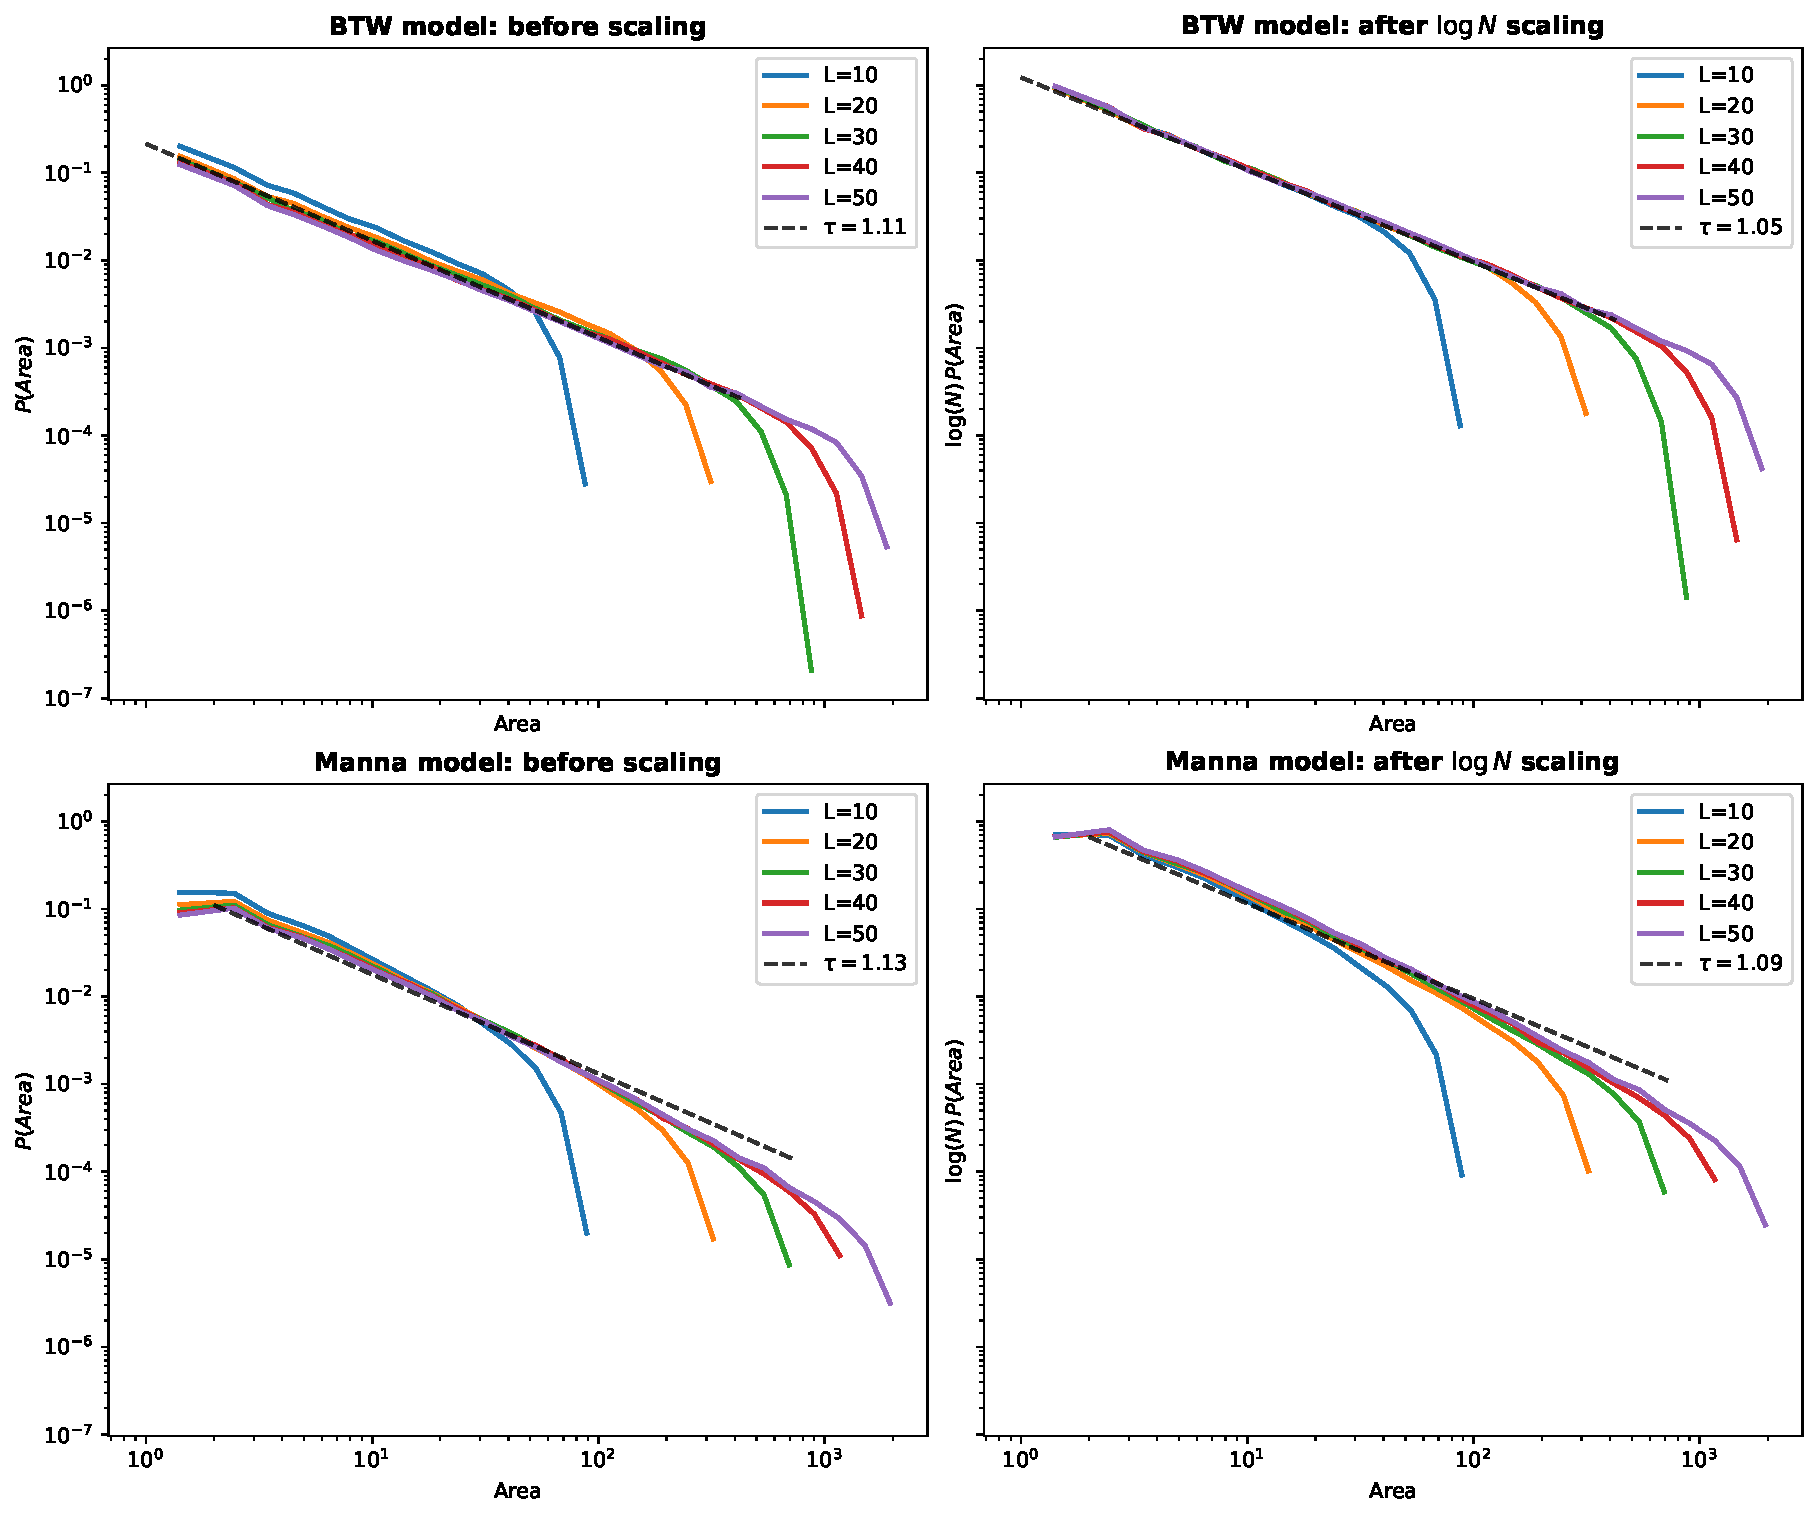
\includegraphics[width=0.80\linewidth]{figures/area.pdf}
    \caption{Log-binned area distributions for the BTW model (top row) and Manna model (bottom row), before scaling (left column) and after $\log N$ scaling (right column).}
    \label{fig:area}
\end{figure}

As shown in Tables \ref{tab:area-summary} and \ref{tab:area-maxdev}, for the BTW model, the area exponent changed from $\tau_a=1.106$ to $\tau_a'=1.054$ after the $\log N$ scaling. The overall RMSE decreased from 0.270 to 0.256, and maximum deviations showed a very similar pattern as in the topples case (substantially decreased for $L=10$ and $L=20$, approximately unchanged for $L=30,40,50$). This may indicate after the rescaling, results from smaller grid sizes show more agreement with the common collapse.

\begin{table}[htbp]
    \centering
    \begin{tabular}{cccc}\toprule
         Model&  $\log N$ scaling&  $\tau$& Overall RMSE\\\midrule
         BTW&  before&  1.106& 0.270\\
         &  after&  1.054& 0.256\\
         Manna&  before&  1.133& 0.365\\
         &  after&  1.088& 0.358\\ \bottomrule
    \end{tabular}
    \caption{Common power-law exponent estimates and overall RMSEs (in log scale) for the area distributions.
}
    \label{tab:area-summary}
\end{table}

For the Manna model, the corresponding exponent estimated decreased from 1.133 to 1.088, RMSE from 0.365 to 0.358. In constrast to the topple case, the maximum deviations mainly remained approximately unchanged or decreased substantially for smaller $L$ values. 

\begin{table}[htbp]
    \centering
    \begin{tabular}{cccclll}\toprule
         Model&  $\log N$ scaling&  $L=10$&  $L=20$& $L=30$& $L=40$& $L=50$\\\midrule
         BTW&  before&  0.493&  0.433& 0.659& 0.897& 1.263\\
         &  after&  0.283&  0.282& 0.698& 0.910& 1.252\\
         Manna&  before&  0.324&  0.514& 0.956& 1.764& 1.670\\
         &  after&  0.258&  0.337& 1.047& 1.797& 1.649\\ \bottomrule
    \end{tabular}
    \caption{Maximum absolute log-space residuals for the area distributions.}
    \label{tab:area-maxdev}
\end{table}

Therefore, the effect of the $\log N$ adjustment on the area
distributions differs for the topple distributions, as now for both BTW and Manna models, it modestly improved the collapse for smaller system sizes.


\section{Loss}\label{sec:loss}

Table \ref{tab:loss-summary} reports the probability of zero loss and exponential fitting results. For both models, $P(loss=0)$ increased with $L$. This is reasonable is since the number of boundary sites only increases proportionally with $L$ while our grid size increases with $L^2$. Avalanches in larger systems are therefore less likely to reach an open boundary.\\

The fitted decay rate $\lambda$ generally decreased with $L$, meaning that the positive loss distribution decayed slower for larger systems. The Manna model generally produced smaller zero loss probabilities than the BTW model. This indicates that boundary dissipation occurred more frequently under its stochastic toppling rule.
\begin{table}[htbp]
    \centering
    \begin{tabular}{cccclll}\toprule
         Model&  Statistics&  $L=10$&  $L=20$& $L=30$& $L=40$& $L=50$\\\midrule
         BTW&  $P(loss=0)$&  0.723&  0.766& 0.793& 0.816& 0.826\\
         &  $\lambda$&  0.327&  0.227& 0.163& 0.137& 0.137\\
 & $R^2$& 0.992& 0.953& 0.936& 0.905&0.929\\
         Manna&  $P(loss=0)$&  0.589&  0.676& 0.724& 0.758& 0.785\\
 & $\lambda$& 0.474& 0.252& 0.199& 0.145&0.118\\
         &  $R^2$&  0.994&  0.939& 0.952& 0.930& 0.902\\ \bottomrule
    \end{tabular}
    \caption{Zero-loss probabilities, exponential decay rates, and $R^2$ values for the loss distributions.}
    \label{tab:loss-summary}
\end{table}

Figure~\ref{fig:positive-loss} shows the log probabilities of positive loss together with the fitted exponential models. The
approximately linear trends on log-normal axes produced
relatively high $R^2$ values, ranging approximately from 0.90 to 0.99.

\begin{figure}[htbp]
    \centering
    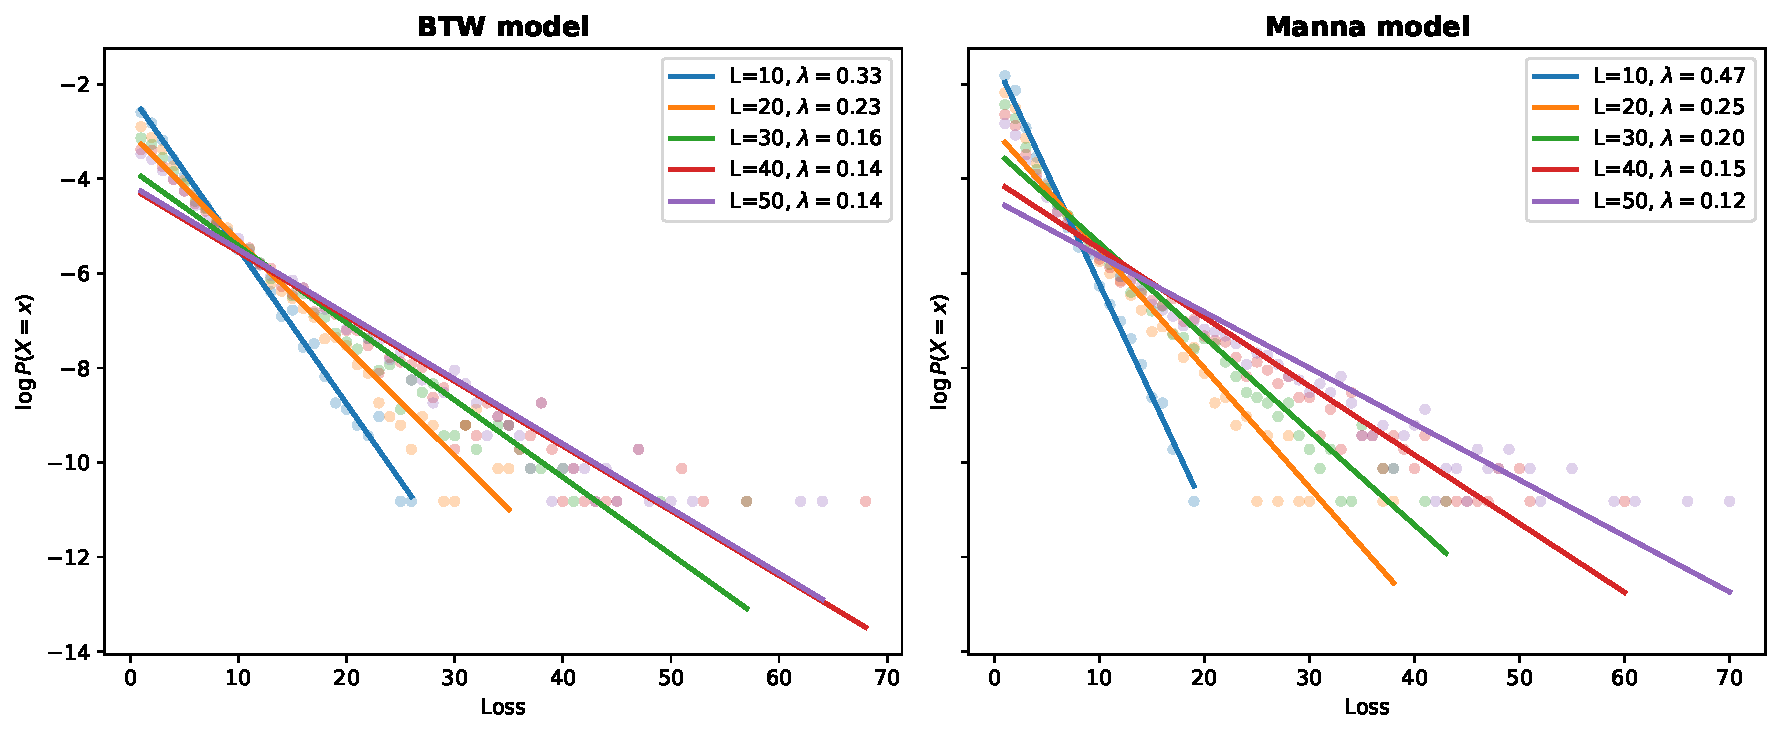
\includegraphics[width=0.80\linewidth]{figures/positive_loss.pdf}
    \caption{Positive loss distributions for BTW model (left) and Manna model (right), with fitted exponential models.}
    \label{fig:positive-loss}
\end{figure}

Nevertheless, Figure~\ref{fig:loss-resid} shows systematic U-shaped residual patterns for most system sizes. Residuals were generally positive for small losses, negative over the intermediate range, and positive again in the far right tail. Thus, the exponential model tends to underestimate the probabilities of small and very large losses while overestimating intermediate probabilities. Therefore, for our limited selected grid sizes $L$, it seems an exponential model may not fully capture the shape of the positive-loss distribution.

\begin{figure}[htbp]
    \centering
    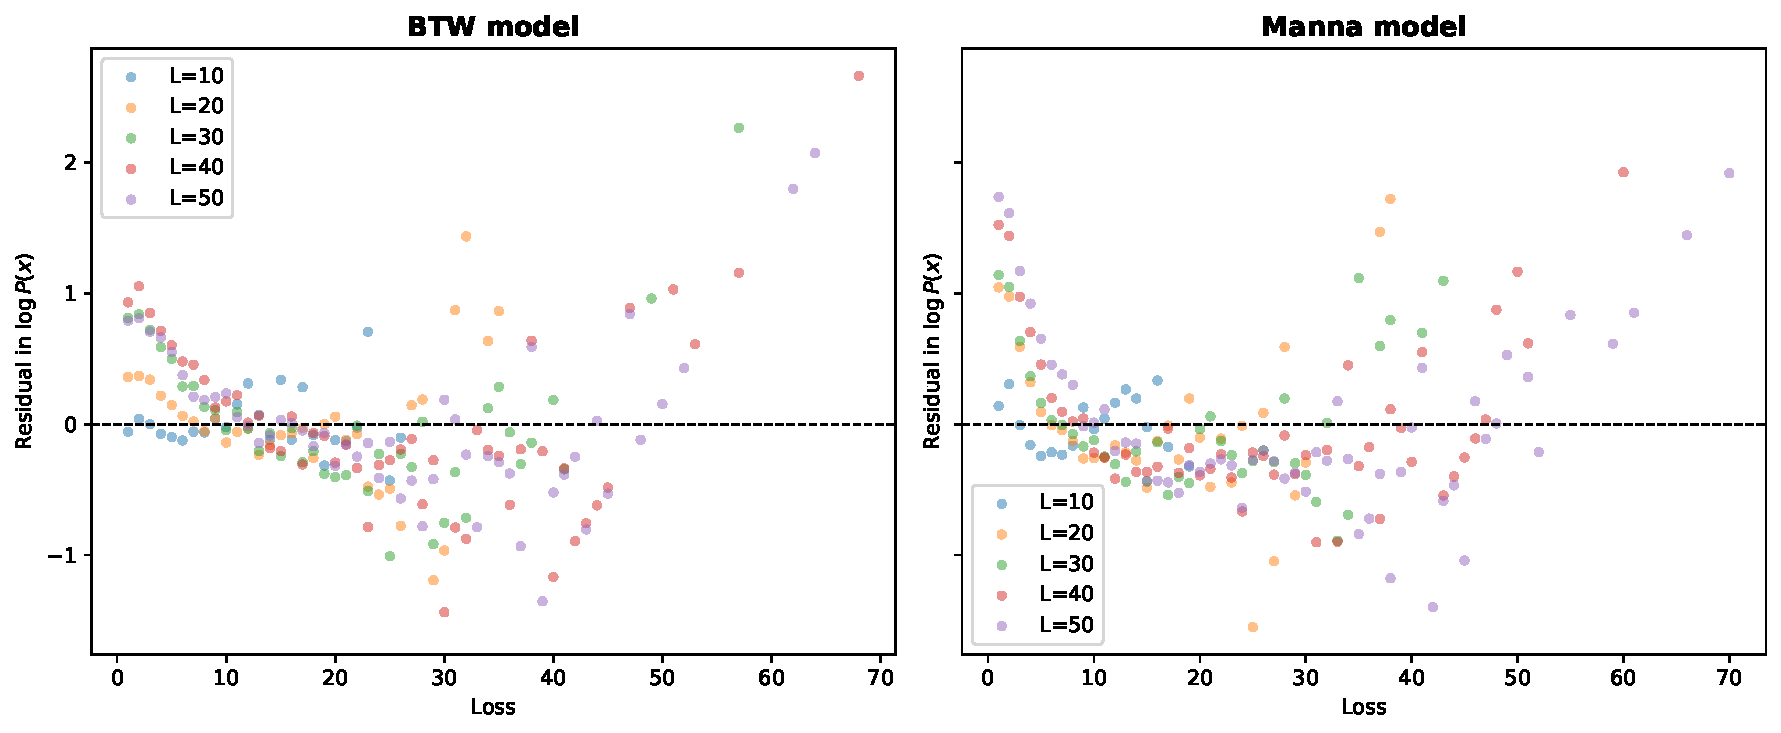
\includegraphics[width=0.80\linewidth]{figures/loss_resid.pdf}
    \caption{Residuals in $\log P(x)$ from the exponential fits for BTW model (left) and Manna model (right). The dashed horizontal line denotes zero residual.
}
    \label{fig:loss-resid}
\end{figure}

\section{Length}\label{sec:equationexamples}

\subsection{Power law}\label{subsec:lengthpowerlaw}

As mentioned in Chapter \ref{ch:methodology}, we lowered the $R^2$ threshold for length because the higher threshold did not identify with a broad enough fitting region. Figure \ref{fig:length-powerlaw} clearly illustrates more visible curvatures within the candidate regions than what we observed for area and topples.\\
\begin{figure}[htbp]
    \centering
    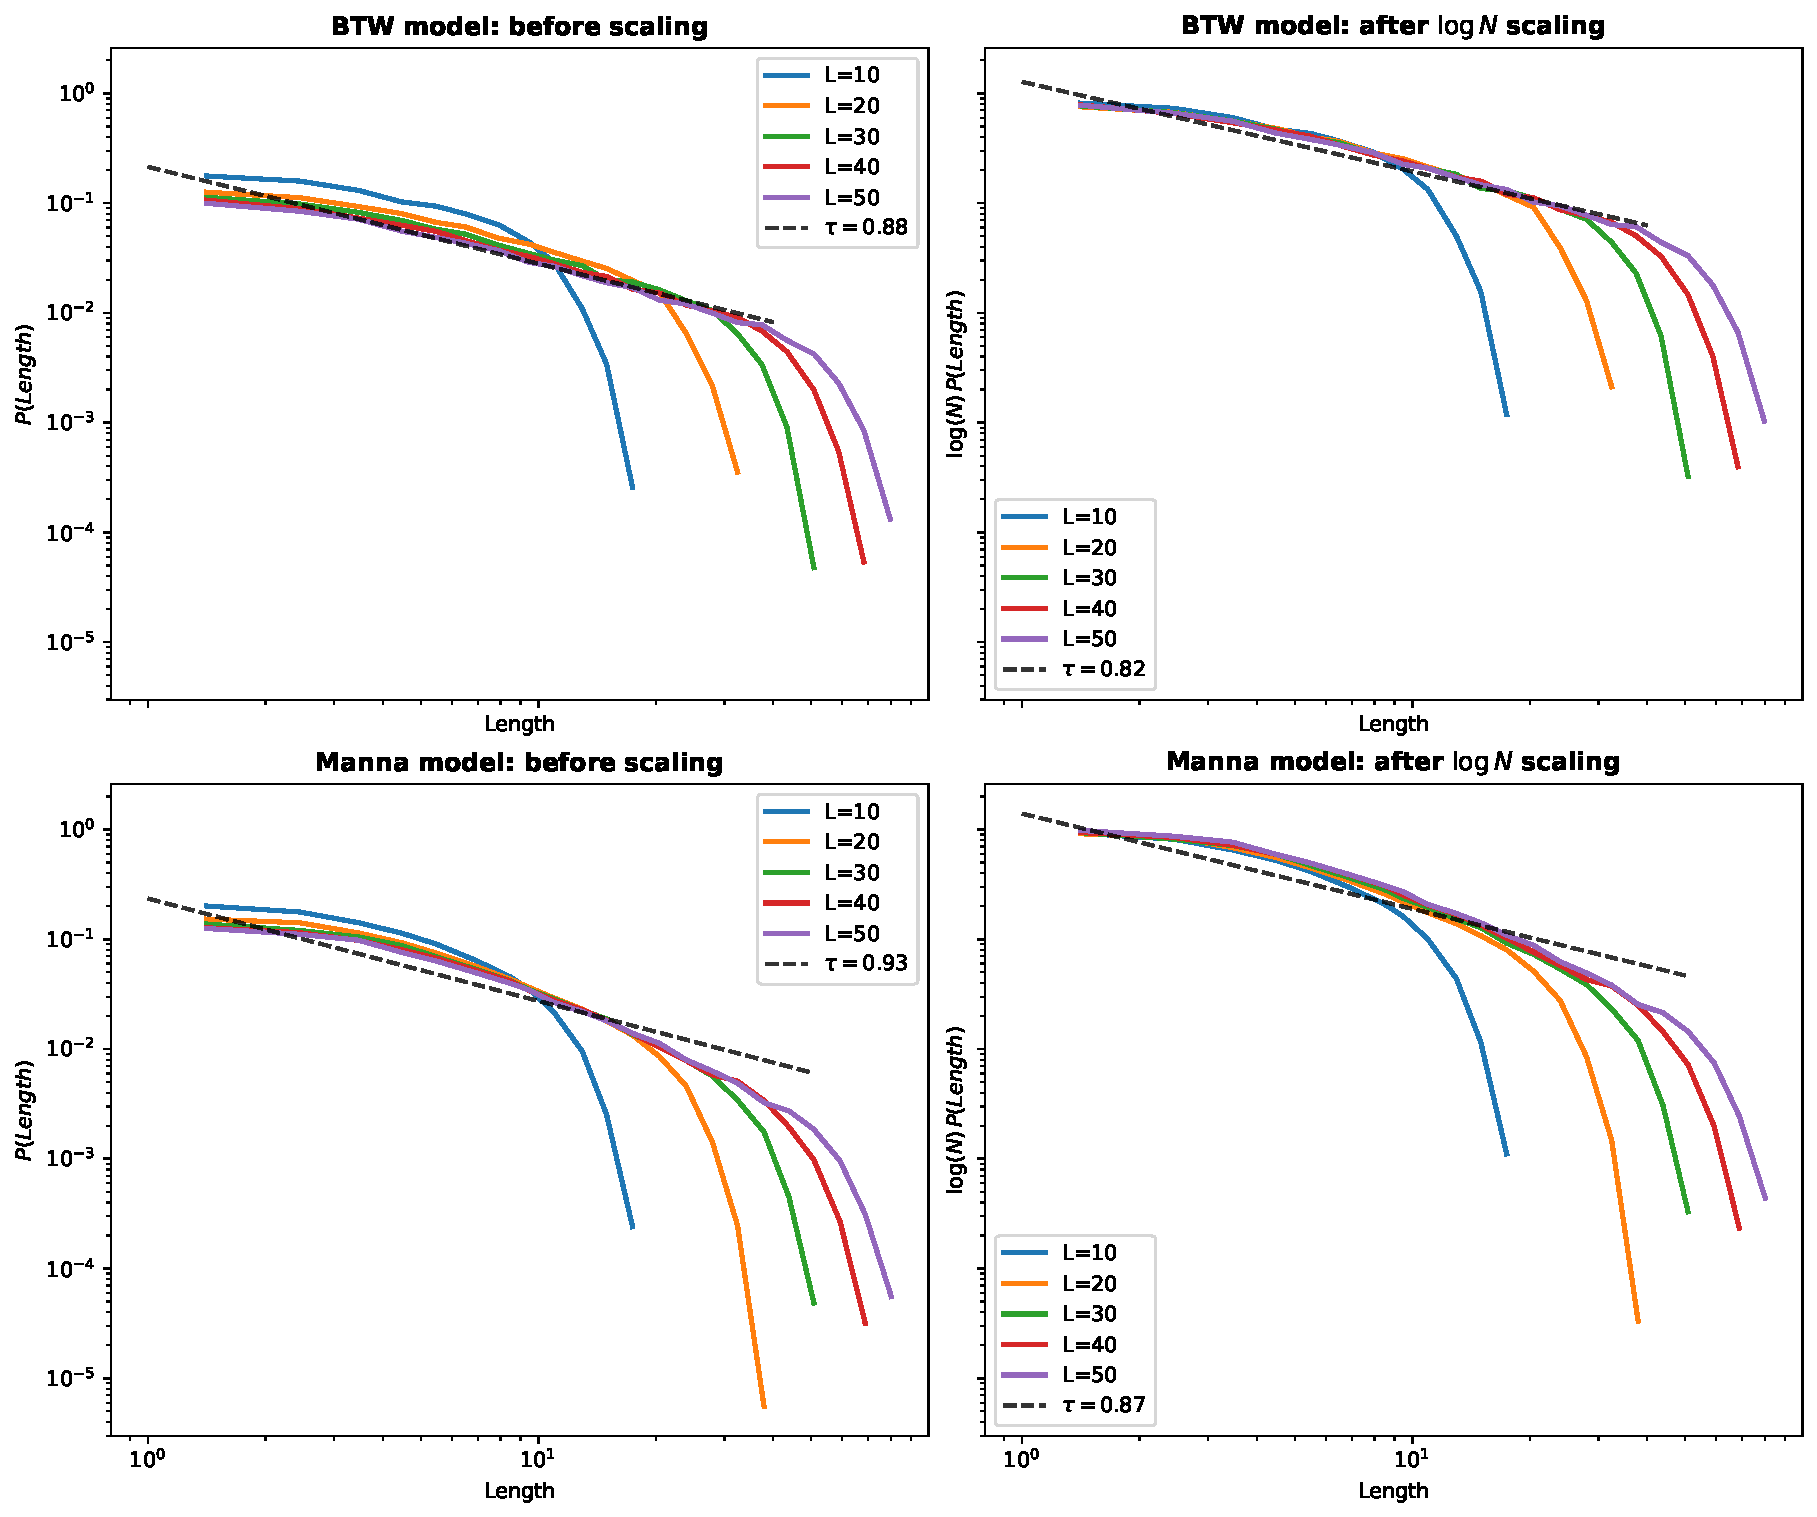
\includegraphics[width=0.80\linewidth]{figures/length_powerlaw.pdf}
    \caption{Log-binned length distributions for the BTW model (top row) and Manna model (bottom row), before scaling (left column) and after $\log N$ scaling (right column).}
    \label{fig:length-powerlaw}
\end{figure}

Table \ref{tab:length-summary-powerlaw} shows that for BTW model, the estimated exponent changed from $\tau_l=0.884$ to $\tau_l'=0.816$ after $\log N$ scaling. The RMSE decreased from 0.223 to 0.152. We may observe a similar pattern in the Manna model, exponent estimates are 0.934 and 0.869 respectively, larger than estimates in BTW model. The RMSE decreased from 0.228 to 0.171. The change is more substantial than the previous cases with area and topples.

\begin{table}[htbp]
    \centering
    \begin{tabular}{cccc}\toprule
         Model&  $\log N$ scaling&  $\tau$& Overall RMSE\\\midrule
         BTW&  before&  0.884& 0.223\\
         &  after&  0.816& 0.152\\
         Manna&  before&  0.934& 0.228\\
         &  after&  0.869& 0.171\\ \bottomrule
    \end{tabular}
    \caption{Common power-law exponent estimates and overall RMSEs (in log scale) for length.
}
    \label{tab:length-summary-powerlaw}
\end{table}

Notably, in both models, maximum deviations in Table  \ref{tab:length-maxdev-powerlaw}  show consistent and generally substantial decrease across all $L$ values after $\log N$ scaling.  Therefore, although the length distributions showed weaker survival function linearity than the topple and area distributions, the common power law fit produced relatively small residuals, and the $\log N$ adjustment substantially reduced the both the overall RMSE and maximum deviations across $L$. This indicates improved alignment between system sizes within the selected fitting regions. 

\begin{table}[htbp]
    \centering
    \begin{tabular}{cccclll}\toprule
         Model&  $\log N$ scaling&  $L=10$&  $L=20$& $L=30$& $L=40$& $L=50$\\\midrule
         BTW&  before&  0.600&  0.532& 0.640& 0.701& 0.766\\
         &  after&  0.446&  0.524& 0.505& 0.484& 0.490\\
         Manna&  before&  0.603&  0.624& 0.732& 0.793& 0.858\\
         &  after&  0.539&  0.616& 0.597& 0.576& 0.583\\ \bottomrule
    \end{tabular}
    \caption{Maximum absolute log-space residuals for length.}
    \label{tab:length-maxdev-powerlaw}
\end{table}

\subsection{Exponential}\label{subsec:lengthexp}

An exponential model was also additionally examined for length because the unscaled distributions displayed visible curvature. However, its residuals exhibited a systematic S-shaped pattern, indicating that a single exponential decay rate did not describe the complete positive-length distribution.\\

\begin{table}[htbp]
    \centering
    \begin{tabular}{cccclll}\toprule
         Model&  Statistics&  $L=10$&  $L=20$& $L=30$& $L=40$& $L=50$\\\midrule
         BTW&  $P(loss=0)$&  0.689&  0.651& 0.633& 0.628& 0.621\\
         &  $\lambda$&  0.417&  0.173& 0.127& 0.093& 0.068\\
 & $R^2$& 0.863& 0.914& 0.889& 0.910&0.920\\
         Manna&  $P(loss=0)$&  0.448&  0.399& 0.381& 0.369& 0.365\\
 & $\lambda$& 0.390& 0.219& 0.138& 0.104&0.085\\
         &  $R^2$&  0.904&  0.909& 0.951& 0.952& 0.960\\ \bottomrule
    \end{tabular}
    \caption{Zero-length probabilities, exponential decay rates, and $R^2$ values for the length distributions.}
    \label{tab:length-summary-exp}
\end{table}

\begin{figure}[!h]
    \centering
    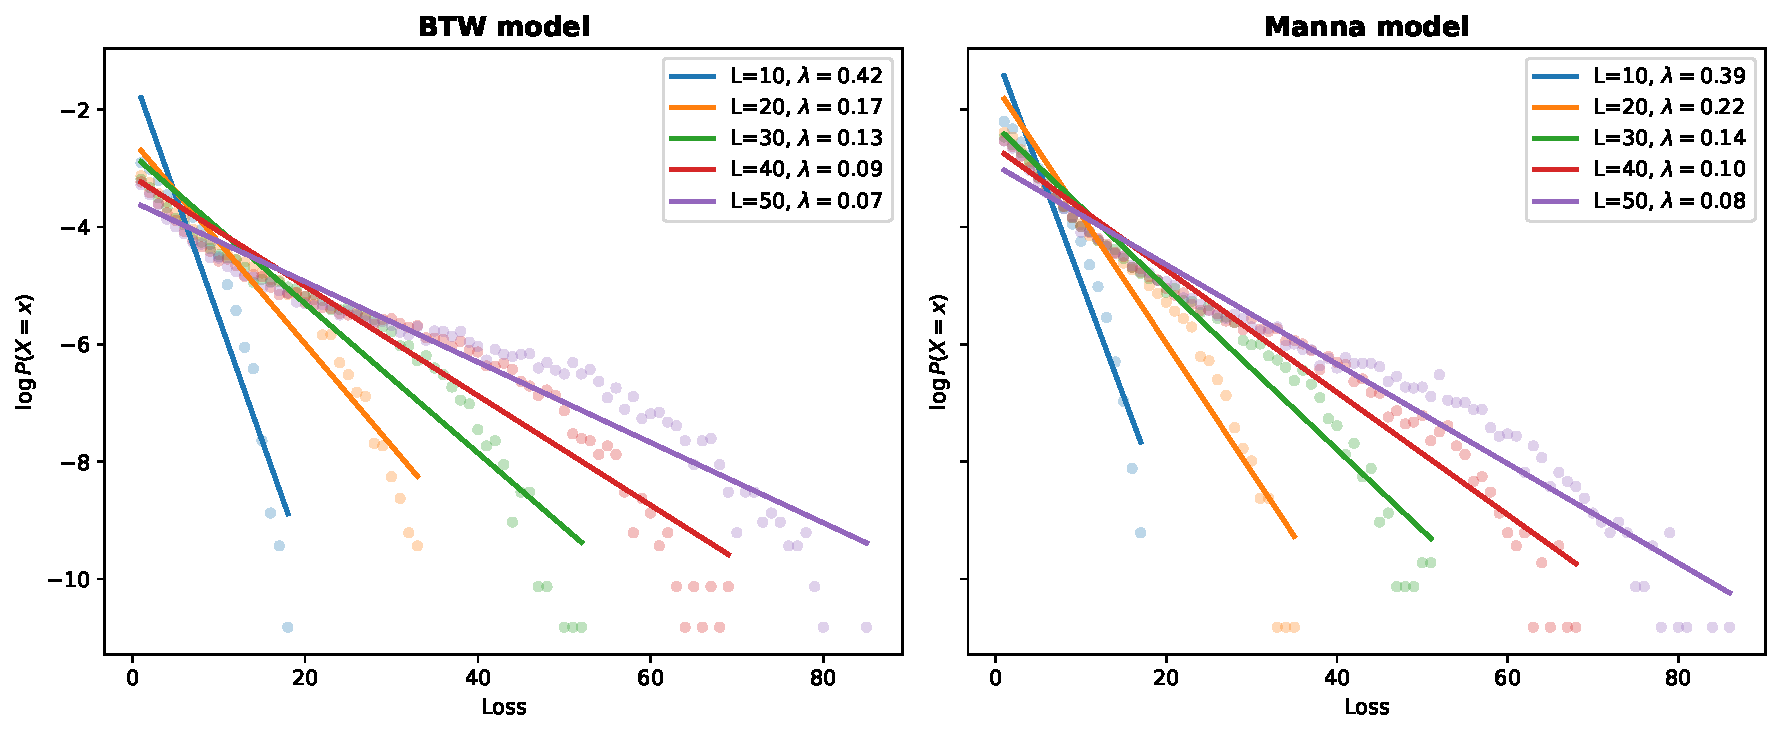
\includegraphics[width=0.80\linewidth]{figures/positive_length.pdf}
    \caption{Positive length for the BTW model (left) and Manna model (right), with fitted exponential models.
}
    \label{fig:positive-length}
\end{figure}

As shown in Figure \ref{fig:positive-length} and Table \ref{tab:length-summary-exp}, the zero loss probability and decay rate both decrease as $L$ increases. This means although zero loss cases became less common, the rate of decay also decreases. This can suggest a broader distribution of positive length.\\

\begin{figure}[htbp]
    \centering
    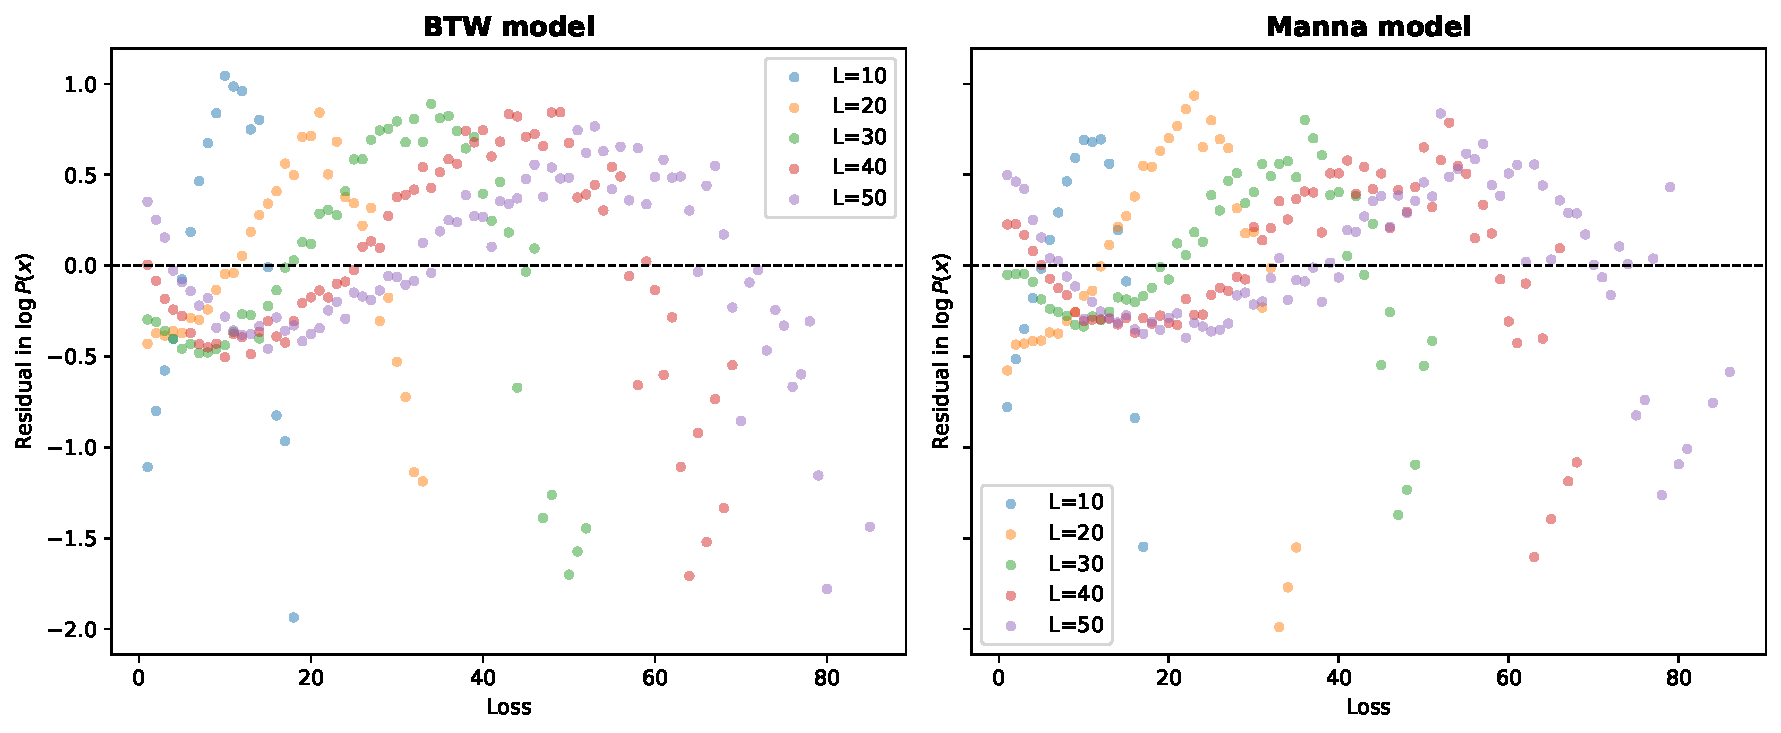
\includegraphics[width=0.80\linewidth]{figures/length_resid.pdf}
    \caption{Residuals in $\log P(x)$ from the exponential length fits for BTW model (left) and Manna model (right). The systematic S-shaped patterns indicate misfit of a single exponential model.
}
    \label{fig:length-resid}
\end{figure}

The diagnostic residual plot in Figure \ref{fig:length-resid} shows a clear S-shaped pattern for most $L$ values. This indicates a systematic misfit of model. That is, a single exponential model does not adequately capture the positive length distribution. We may observe the same curvature in Figure \ref{fig:positive-length} as scattered around the fitted lines. \\

Overall the results may favour an approximate power-law description with FSS, however the evidence is weaker than for topples and area. Neither model fully describes the positive length distribution.

\section{Correlations}\label{sec:correlations}

The pairwise correlations between avalanche observables were measured using Spearman rank correlation. As previously discussed, Spearman correlation was preferred because the data were discrete and strongly right-skewed. The correlations matrix shows small variations in value across $L$ values, we only display the result for $L=50$ here and the rest is left in Appendix \ref{app:correlations}.

\begin{table}[!h]
    \centering
    \begin{tabular}{ccccc}\toprule
         &  Topples&  Area&  Loss& Length\\\midrule
         Topples&  1.000&  -&  -& -\\
         Area&  1.000&  1.000&  -& -\\
         Loss&  0.626&  0.626&  1.000& -\\
         Length&  0.963&  0.964&  0.625& 1.000\\ \bottomrule
    \end{tabular}
    \caption{Pairwise Spearman's correlation for the BTW model, $L=50$}
    \label{tab:corrBTW50}
\end{table}

\begin{table}[!h]
    \centering
    \begin{tabular}{ccccc}\toprule
         &  Topples&  Area&  Loss& Length\\\midrule
         Topples&  1.000&  -&  -& -\\
         Area&  0.999&  1.000&  -& -\\
         Loss&  0.527&  0.527&  1.000& -\\
         Length&  0.982&  0.984&  0.516& 1.000\\ \bottomrule
    \end{tabular}
    \caption{Pairwise Spearman's correlation for the Manna model, $L=50$}
    \label{tab:corrManna50}
\end{table}

The result is consistent as what we have discussed previously in Section \ref{sec:properties}. Topples, area and length are strongly and positively correlated for both models. Correlations involving loss were positive but noticeably weaker, since loss depends specifically on whether an avalanche reaches the open boundary.
